\chapter{作品概述}

\section{功能与特性}

TriHaRiscv\footnote{TriHaRiscv的命名灵感来源于团队名称“哈哈哈”（即Triple Ha）。}是基于自研RISC-V CPU与NPU的异构视觉处理系统。
设计以CPU实现、国产FPGA集成及性能分析为主线，通过人脸检测和预设人物头像叠加展示处理器、计算加速和视频处理的协同工作。
系统在盘古100pro+平台上集成CPU、NPU、AXI互连、存储及HDMI视频链路，具备以下功能与特性：
\begin{itemize}
    \item CPU采用六级流水线、单发射、顺序执行与顺序提交结构，支持RV32IM指令集、CSR访问及\texttt{FENCE.I}指令。
    \item CPU运行于机器模式，支持异常处理、中断响应与返回，提供周期计数；仿真通过WB提交观测与流水线事件分析执行效率。
    \item I-Cache与D-Cache各为16\,KiB，采用两路组相联、32\,B缓存行；D-Cache采用写回、写分配策略，支持缓存行清理与失效。
    \item 动态分支预测采用512项两位计数器BHT、512项直接映射BTB和4项返回地址栈；64\,bit取指包与两项取指FIFO为单发射流水线供给指令。
    \item NPU采用INT8乘法、INT32累加，提供64和128乘加通路配置，支持普通卷积、逐点卷积、深度卷积及网络所需辅助算子。
    \item CPU按算子配置NPU，NPU在内部完成分块循环；DMA搬运权重、特征图和计算结果，完成通知与输出写响应保持一致。
    \item 采用32\,bit AXI4-Lite控制接口和128\,bit AXI4数据DMA接口，通过桥接连接CPU访存接口与DDR控制器。
    \item 集成Boot ROM、片上SRAM及1\,GB板载DDR3，划分CPU私有可缓存区和DMA不可缓存共享区。
    \item 集成UART、GPIO、定时器、SPI、I\textsuperscript{2}C和外部中断控制，支持程序装载、板级初始化及运行状态记录。
    \item HDMI输入与输出均为800$\times$600、标称60\,Hz，检测覆盖完整输入画面，显示端按帧切换RAW、BOX和AVATAR全屏模式。
    \item 视频硬件生成400$\times$300 RGB888预览图和320$\times$320 UINT8 BGR NCHW输入，完成双线性缩放、补边、行缓冲、头像映射及Alpha混合，CPU提交帧地址及显示参数。
    \item 裸机运行YuNet人脸检测，CPU完成定点解码、NMS和主人脸选择，三帧槽管理采集、处理和显示的数据生命周期。
\end{itemize}

\section{应用领域}

系统面向交互式视觉终端、数字镜面和嵌入式视觉等场景。输入视频经YuNet检测后，显示端在完整原图上叠加人脸框、关键点或主人脸对应的预设动漫头像。
用户通过MODE按键切换原图、检测标记和头像叠加三种全屏模式，切换在有效图像起点生效。
主人脸按有效框面积、置信度及固定候选顺序选择，头像由软件配置，叠加采用二维缩放、平移与透明混合。

模型准备和素材转换在主机离线完成。程序、权重和素材装载后，FPGA独立执行图像处理、网络推理、检测后处理和视频输出。
同一硬件平台还用于CPU指令集验证、Cache与分支预测分析，以及CPU、NPU和视频DMA并发访问DDR时的系统性能研究。

\section{主要技术特点}

\begin{itemize}
    \item 六级单发射CPU将取指请求与指令返回分开，通过旁路、停顿和冲刷处理相关性与控制转移，配合Cache和动态分支预测减少执行等待。
    \item CPU、NPU和Video按计算粒度分工：CPU执行控制与有限候选后处理，NPU执行卷积和张量运算，Video执行逐像素预处理及显示合成。
    \item 普通卷积与深度卷积采用不同的数据组织方式，结合局部缓冲、跨通道块部分和保存和DMA搬运，提高乘加通路的有效利用率。
    \item 原图、预览图、模型输入及结果按帧绑定，显示地址和叠加参数在有效图像边界整体切换，旧槽在读事务、行缓冲及像素引用退休并完成释放确认后复用。
    \item 显示端按行读取原分辨率底图，在像素流水中完成框、关键点及头像合成，合成结果直接输出，省去整帧叠加图的DDR写回。
\end{itemize}

\section{设计流程}

本设计以自研RISC-V CPU的实现、国产FPGA验证及性能分析为目标，以YuNet人脸检测和单HDMI全屏头像叠加作为系统应用。
开发分为CPU、NPU和Video三条并行路线，分别完成独立验证与板级集成，再通过统一的地址、寄存器和帧接口连接，整体流程如图\ref{fig:design-flow}所示。

\begin{figure}[!htbp]
\centering
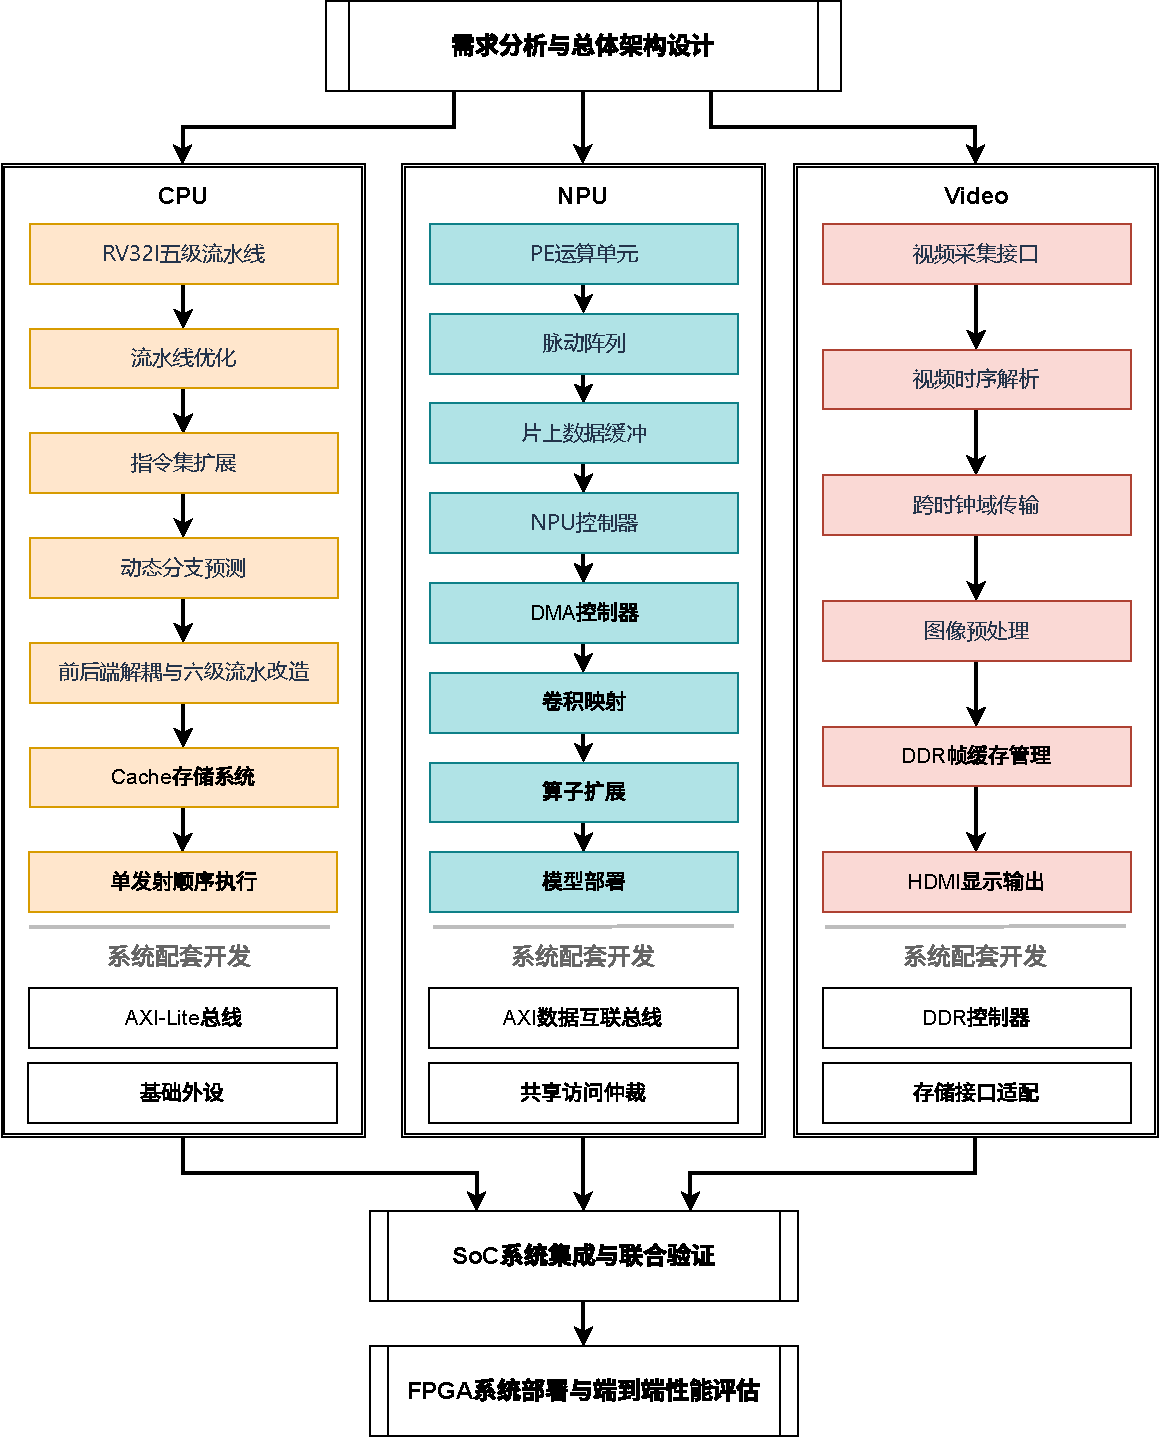
\includegraphics[width=\linewidth,height=0.78\textheight,keepaspectratio]{../figure/rv32-soc-page4.pdf}
\caption{TriHaRiscv设计流程}\label{fig:design-flow}
\end{figure}

\begin{enumerate}
    \item CPU路线完成六级单发射流水线、指令集、Cache、分支预测及异常中断设计，集成SoC互连与外设，
    实现定点检测后处理和帧调度。CoreMark、IPC及资源和时序分析贯穿各个可运行版本。
    \item NPU路线围绕固定YuNet计算图完成算子审计、量化和整数参考，设计PE、普通与深度卷积通路、片上缓冲及DMA，
    配套辅助算子和逐层数值核对，形成软件可调度的计算硬件与模型包。
    \item Video路线完成HDMI接收与发送、全帧采集、预览降采样及模型输入双线性缩放，设计三帧槽、输入格式化、显示行缓冲和头像叠加，
    通过显示记录提交、实际像素生效及旧帧释放确认连接软件调度和连续视频扫描。
\end{enumerate}

系统配套开发统一了DDR封装、AXI互连、时钟复位和公共配置。CPU负责互连和软件集成，Video负责DDR与像素域封装，
NPU提供计算接口、整数语义和模型数据。各路线通过CPU与NPU静态推理、CPU与Video控制、预处理与整数参考核对完成子系统联合验证。

FPGA部署将处理器、计算加速和视频链路集成到PG2L100H-6IFBG676，完成时钟、引脚和接口约束配置。
CPU性能采用CoreMark、CoreMark/MHz、CoreMark/LUT和IPC统计；FPGA实现分析最高工作频率（Fmax）与LUT、FF、DRM和APM资源占用。
应用端到端性能评估统计有效输出帧率、板内可见延迟、更新间隔及丢帧，结合逐层计算、DDR等待和CPU后处理定位开销。
